\documentclass[a4paper,10pt]{article}
\usepackage[utf8]{inputenc}
\usepackage{url}
\usepackage{amsthm, amscd, amsfonts, amssymb, graphicx,tikz, color, environ}

%opening
\title{Literature Review: Simulating Flexible Assembly System Event Logs for the Purposes of Process Modelling and Machine Learning – DRAFT}
\author{Tero Keski-Valkama}

\begin{document}

\maketitle

\smallskip
\noindent \textbf{Keywords.} Anomaly detection, Assembly system, Fault detection, Long short-term memory

\section{Description of Method}

This is a literature review of the first phase of the research, which is about simulating industrial assembly processes and faults for the purposes of
process modelling and machine learning research.

A proper literature review is a methodological, continuous process. The goal of the literature review is to accumulate a body of relevant existing knowledge
about the topic, categorized based on subtopics and keywords.
Ultimately the literature review can be presented in the article in a summary form to present the context of the research.
The collected references represent a focused area of the existing literature relevant to the object of research.

The review starts from discovery, discovering information sources and starting points of review. The literature review process progresses towards synthesis
where the relevant existing knowledge is synthesized together to form an understanding of the composite.

The discovery phase includes a listing of subtopics and keywords, to structure the gathered discovered information into a manageable form. The goal
of the discovery phase is to form questions about the existing knowledge and to find answers to them.

The synthesis is composed of the description of the existing knowledge and possible gaps related to the research.

\section{Discovery Phase}

The topic under review is somewhat cross-discplinary relating to industrial assembly processes, business process modelling and learning systems.
Overall the following subtopics are recognized:
\begin{enumerate}
 \item Assembly process modelling and simulation
   \begin{enumerate}
     \item Fault modelling and simulation
   \end{enumerate}
 \item Mathematical analysis of log data
   \begin{enumerate}
     \item Analysing interleaved event streams
     \item Analysing delays and intervals
   \end{enumerate}
 \item Process mining
 \item Visualization of event logs
\end{enumerate}

\begin{figure}[h]
\begin{center}
 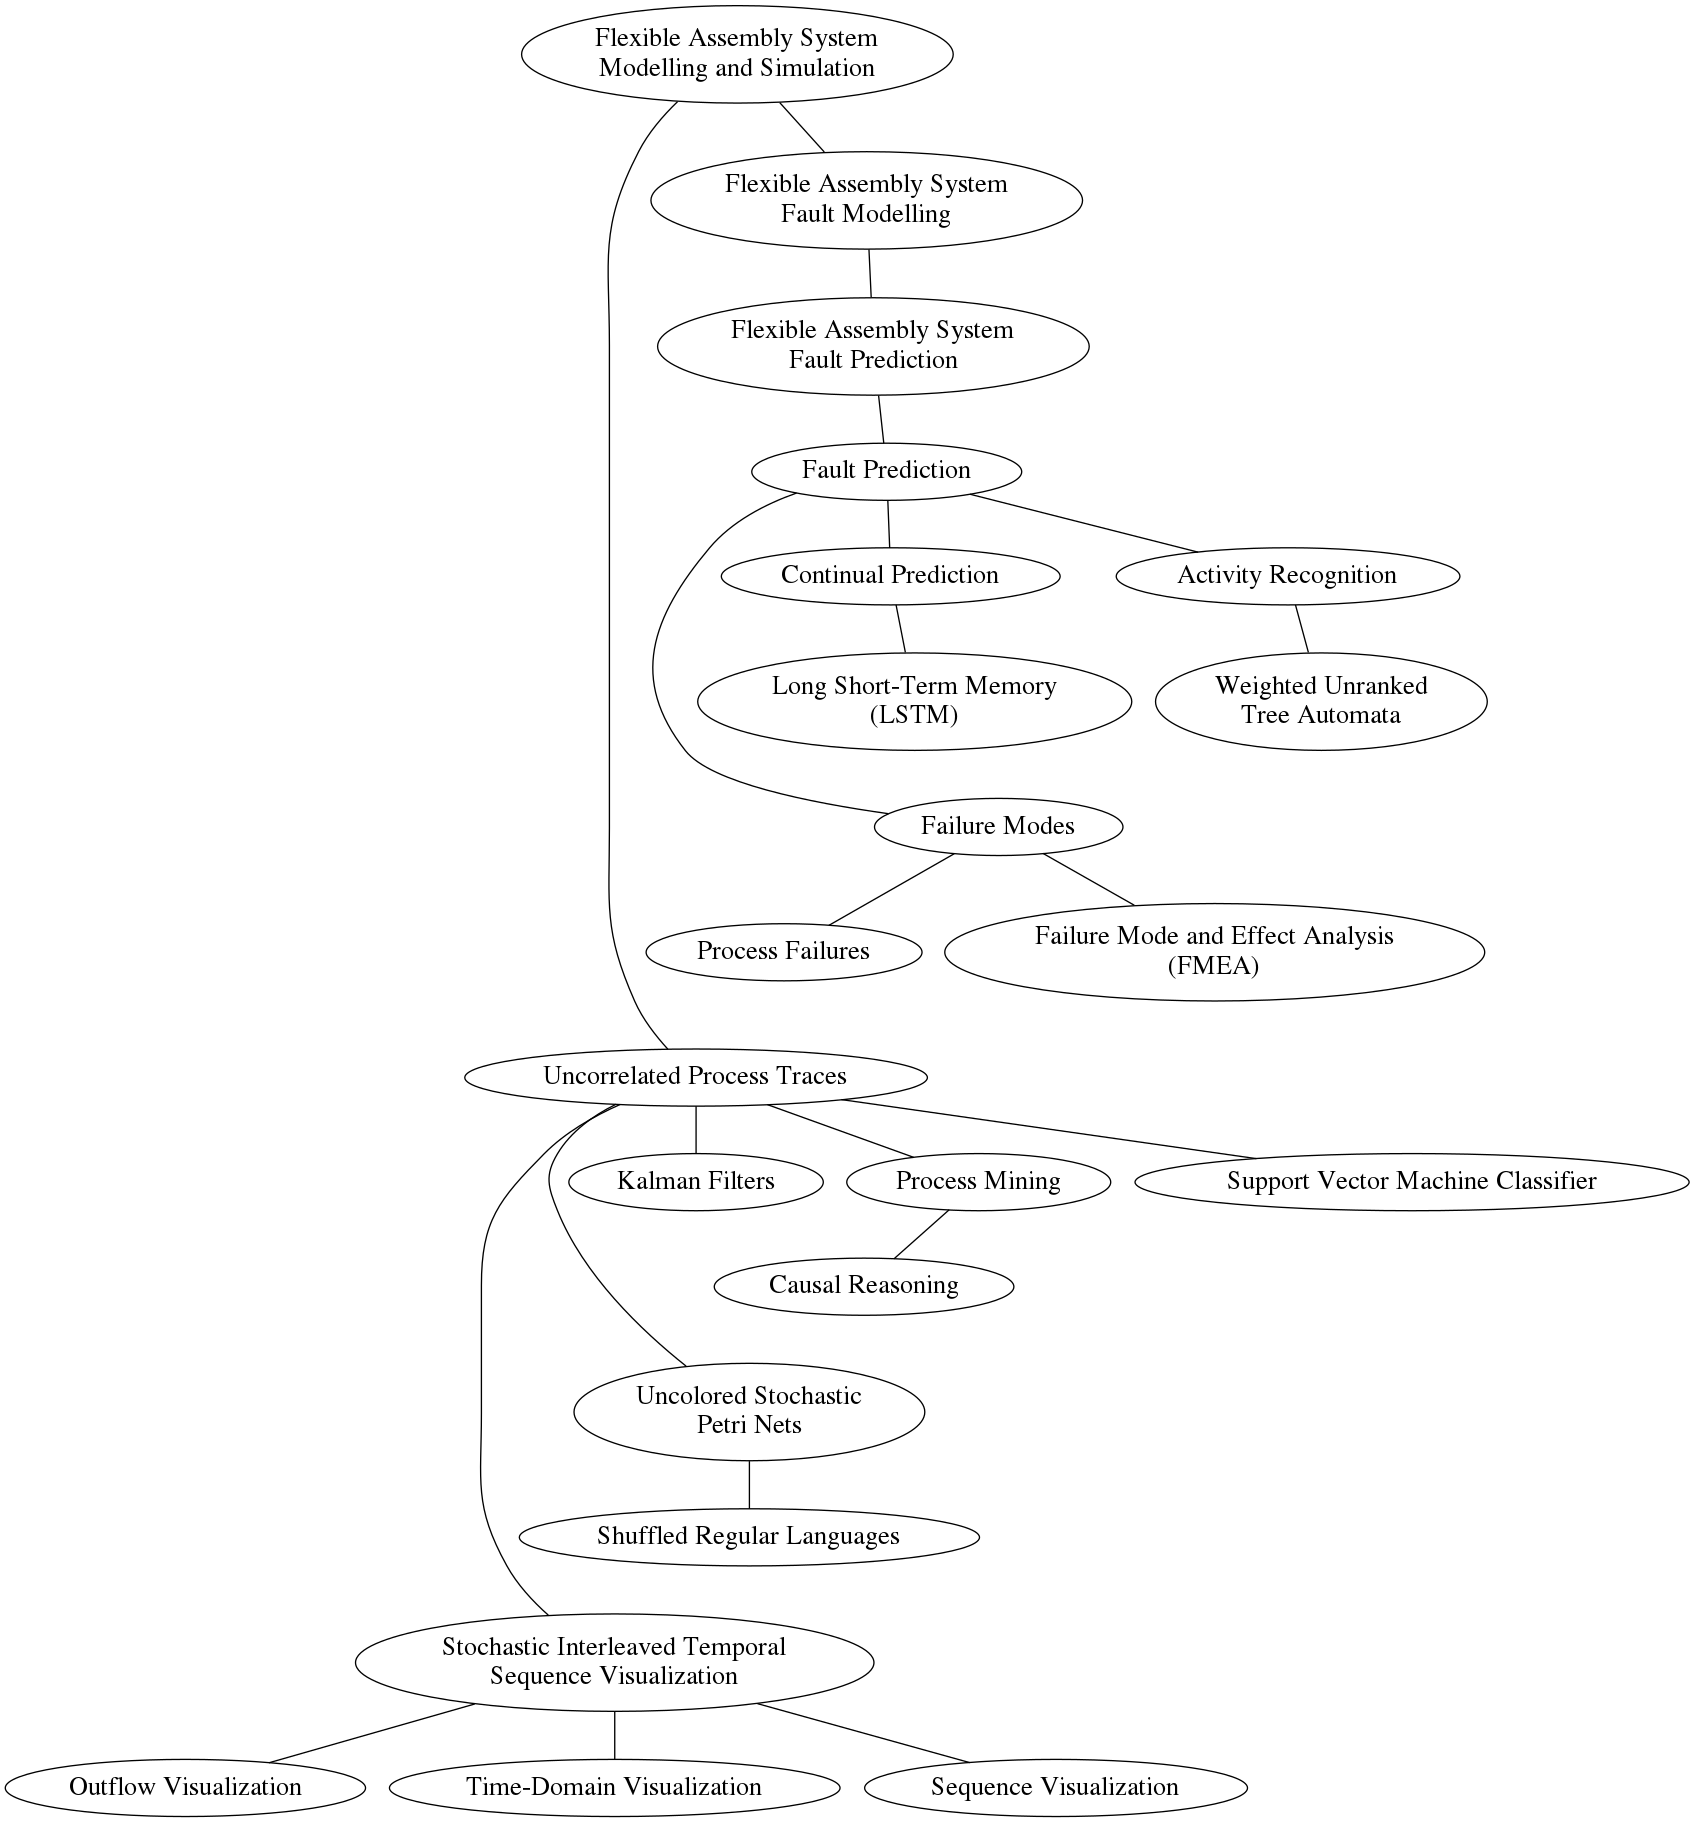
\includegraphics[width=\textwidth]{./field.png}
 % field.png: 0x0 pixel, 300dpi, 0.00x0.00 cm, bb=
\end{center}
\caption{The mind map of the research topic}
\end{figure} 

\subsection{Keywords}

The keywords relevant for the research were collected from a set of articles deemed especially relevant for this research. A representative set of articles was
read and relevant keywords were picked from titles, abstracts and references. This set of keywords allows for directed browsing of relevant literature.

\begin{itemize}
 \item activity recognition
 \item alpha algorithm
 \item anomaly detection
 \item assembly process
 \item assembly system
 \item bidirectional LSTM
 \item causal reasoning
 \item complex robotic system
 \item compliant parts
 \item Connectionist Temporal Classification
 \item context-free languages
 \item continual prediction
 \item Convolutional Neural Network
 \item corpus
 \item Deep Recurrent Neural Networks
 \item dimensional quality
 \item dimensional variation propagation
 \item extended hybrid petri nets
 \item Failure mode and effects analysis (FMEA)
 \item failure rates
 \item failure records
 \item failure report
 \item fault detection
 \item fault mode
 \item fixture variation
 \item fuzzy generalized stochastic petri nets
 \item interleaving
 \item kalman filters
 \item keyhole plan recognition
 \item knowledge modelling
 \item labelling unsegmented sequence data
 \item leaf spring
 \item learning Context Sensitive Languages
 \item Long Short-Term Memory (LSTM)
 \item multiple failure modes
 \item Multi-Station Assembly Systems
 \item nonregular languages
 \item outflow visualization
 \item part variation
 \item petri nets
 \item plan recognition
 \item process control
 \item process failures
 \item process FMEA
 \item reduction of irregularities
 \item reliability
 \item shuffled languages
 \item shuffle languages
 \item shuffle of regular languages
 \item simulation
 \item Stochastic Petri Nets
 \item Support Vector Machine classifier
 \item system verification
 \item time-domain visualization
 \item variation propagation
 \item visualization of sequences
 \item Weighted Unranked Tree Automata
 \item welding gun variation
\end{itemize}

The core questions about the existing literature are:
\begin{enumerate}
 \item What are the current best methods of industrial event log based anomaly detection or process mining?
 \item What methods are there to model and simulate assembly processes and related faults?
 \item What methods are there to visualize event logs with or without timestamps?
 \item What methods are there to mathematically model logs generated by parallel processes, or shuffled languages?
 \item What are the relevant keywords and terms to describe this problem space?
\end{enumerate}

\section{Synthesis}

Process mining is the field of inferring the underlying business processes based on observer events and transitions.
The current de facto methods for describing process logs in the context of process mining are based on the alpha algorithm and they all expect process instances
to be identified in the input event streams.

\end{document}


